\section{Josip Osti}

\begin{verse}

\textbf{Kadarkoli se srečava, se dolgo gledava}

\medskip

Kadarkoli se srečava, se dolgo gledava\dots\\
Ko se nepričakovano srečava na poti,\\
ki pelje skoz gozd ali vinograd, in tudi \\
ko se mi v vrtu skoz travo, prepolno \\
regratovih cvetov, podobnih zvezdam,\\
bliža gola. Z gibkimi gibi. Popolnoma\\
neslišno, kot da gre po prstih. V njenih \\
lepih očeh, iz katerih veje hlad\\
najglobljega vodnjaka, vsakič vidim svoje \\
oči in v njih podvojeno pekoče sonce. \\
Ne vem, ali tudi ona čuti mojo veliko \\
željo kot jaz njeno, da bi se vsaj enkrat \\
strastno poljubila. \dots Kadarkoli se srečava, \\
se dolgo gledava. \dots Tako se konča vsako \\
moje srečanje s kačo. \\

\bigskip
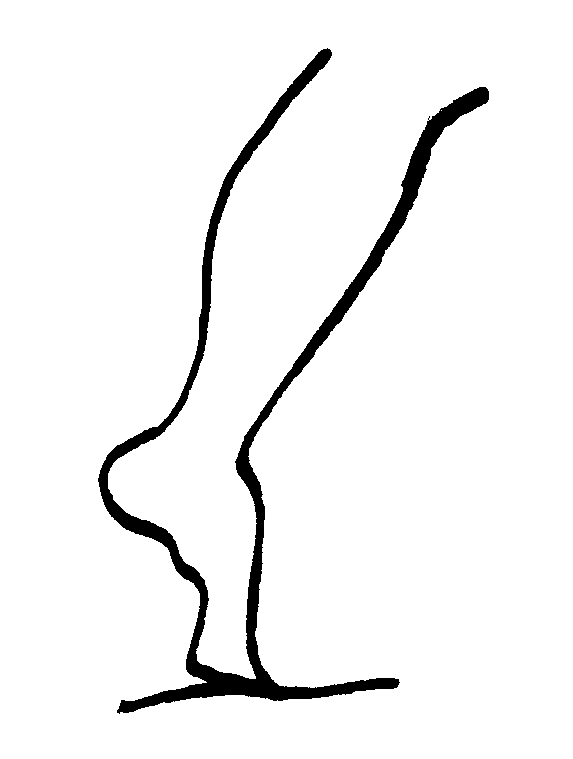
\includegraphics[width=6cm,height=7cm]{plavrevue-30/img/kdykoliv.png}
\bigskip

\textbf{Kdykoli se setkáme, dlouho na sebe hledíme}
\medskip

Kdykoli se setkáme, dlouho na sebe hledíme\ldots \\
Když se nečekaně setkáme na cestě, \\
která vede lesem nebo vinicí a také \\
když se ke mně v zahradě travou, plnou \\
květů pampelišky, podobných hvězdám, \\
blíží holá. Hladkými pohyby. Úplně \\
neslyšně, jako by našlapovala po špičkách. \\
V jejích krásných očích, z nichž vane chlad \\
nejhlubší studně, pokaždé vidím své \\
oči a v nich zdvojené žhnoucí slunce. \\
Nevím, jestli i ona cítí moji velkou  \\
touhu jako já její, abychom se aspoň jednou \\
vášnivě políbili\ldots Kdykoli se setkáme, \\
dlouho na sebe hledíme\ldots Tak končí každé \\
mé setkání se zmijí.


\medskip

\podpis{přeložil Aleš Kozár}

\end{verse}



